\documentclass{article}
\usepackage[utf8]{inputenc}
\usepackage[margin=1in]{geometry}
\usepackage{amsmath}
\usepackage{braket}
\usepackage{bbold}
\usepackage{graphicx}
\usepackage{import}
\usepackage{xifthen}
\usepackage{pdfpages}
\usepackage{transparent}

\newcommand{\incfig}[1]{%
    \def\svgwidth{\columnwidth}
    \import{./Figures/}{#1.pdf_tex}
}
\graphicspath{{./Mathematica/}}
\title{Tunnelling Times in Quantum Mechanics}
\author{James Puleston}

\begin{document}

\maketitle

\section{Time in Quantum Mechanics}

\subsection{Time in Classical Mechanics}
In the Hamiltonian formulation of classical mechanics, a system with $n$ degrees of freedom possesses $2n$ independent first-order differential equations in terms of $2n$ independent variables. These variables are the coordinates of the \textit{phase space} of the system, and the $2n$ equations of motion describe the evolution of system in the phase space. $n$ of the independent variables are conventionally chosen to be the generalised coordinates $q_i$ and the other $n$ set to be the conjugate momenta $p_i$, which obey the Poisson bracket relations: \cite{Goldstein}

\begin{equation}
	\{q_i, p_j\}=\delta_{ij} \quad \{q_i, q_j\}=\{p_i,p_j\}=0, \quad i,j=\{1,\dots,n\}
	\label{conjugatevars}
\end{equation}

\noindent The time evolution of the canonical variables is governed by the Hamiltonian $H = H(q_i, p_i)$:

\begin{equation}
	\frac{dq_i}{dt} = \{q_i, H\} \quad \frac{dp_i}{dt} = \{p_i, H\}
	\label{timeevolution}
\end{equation}

\noindent For an infinitesimal variation in time, $\delta t = \delta \tau$, the associated variation in the dynamical variables is:

\begin{equation}
	\delta q_i = \{q_i, H\}\delta\tau \quad \delta p_i = \{p_i, H\}\delta\tau
	\label{timetranslation}
\end{equation}

\noindent $q_i$ and $p_i$ are generalised variables; they are not necessarily positions and momenta, but in the case of a dynamical system comprised of a collection of point particles, the canonical variables are usually the particles' positions $(\boldsymbol{q_i})$ and momenta $(\boldsymbol{p_i})$. 

In classical mechanics, physical systems are embedded in a 4-dimensional continuous space-time background, the points of which are assigned coordinates $(t,x,y,z) = (t, \boldsymbol{x})$.
It is essential that the \textit{definitions} of these two spaces and their associated coordinates are not conflated. In particular we must distinguish the position variable $\boldsymbol{q}$ from the space-time coordinate $\boldsymbol{x}$. The former defines a point in the phase space of the system (when accompanied by its associated momentum $\boldsymbol{p}$) and is a property of a point particle, whereas the latter is the coordinate of a fixed point in the space-time background in which the dynamical system is embedded. Note we can still introduce both sets of quantities in to equations and relate them, as equations (\ref{timeevolution}) and (\ref{timetranslation}) show.

Immediately this raises the question of whether there exists physical systems that possess a dynamical variable that \textit{resembles} the time coordinate of space-time. Such systems are called \textit{clocks}, more precisely defined as physical systems with a dynamical `clock' or `time' variable that behaves similarly to the space-time time coordinate $t$ under time translations. For example, under time translation in which the space-time coordinates transform as:

\begin{equation}
\boldsymbol{x} \rightarrow \boldsymbol{x} \quad t \rightarrow t+\tau
\label{timetranslation2}
\end{equation}

\noindent a \textit{linear} clock variable $\theta$ and its conjugate momentum $\eta$ transform as:

\begin{equation}
	\eta \rightarrow \eta \quad \theta \rightarrow \theta + \tau
	\label{timetranslation3}
\end{equation}

\noindent Comparing with (\ref{timetranslation}) we see in the infinitesimal case of (\ref{timetranslation3}):

\begin{equation}
	\delta\eta=\{\eta, H\}\delta\tau \quad \delta\theta = \{\theta, H\}\delta\tau
	\label{timetranslation4}
\end{equation}

\noindent which implies

\begin{equation}
	\{\eta, H\}=0 \quad \{\theta, H\}=1
	\label{timetranslation5}
\end{equation}

\noindent The equation of motion given by (\ref{timeevolution}), $\frac{d\theta}{dt}=1$ has solution $\theta=t+t_0$.

\subsection{Time in Quantum Mechanics}
In quantum mechanics we describe a system of $N$ particles using a wave function which represents the quantum state of the system. The domain of a time-dependent wave functions $\psi(\boldsymbol{q_1},\dots,\boldsymbol{q_N}, t)$ is $\mathbb{R}^{3N}\times\mathbb{R}$, where $\mathbb{R}^{3N}$ is the \textit{configuration space} of the system. All possible quantum states reside in a Hilbert space referred to as the \textit{state space} of quantum mechanics. We use canonical quantisation to evolve the Hamiltonian formalism of classical mechanics into a quantum theory. Under this process, dynamical variables are promoted to operators on Hilbert space (`quantised'), and Poisson brackets replaced by commutation relations according to:

\begin{equation}
\{,\} \rightarrow \frac{1}{i\hbar}[,]
\end{equation}

\noindent Following this prescription, (\ref{conjugatevars}) becomes:

\begin{equation}
	[q_i,p_j]=i\hbar\delta_{ij} \quad [q_i,q_j]=[p_i,p_j]=0
\end{equation}

The time variable does not undergo canonical quantisation - it remains a c-number that acts as a parameter in the theory. This raises the question of why time and position are treated differently in quantum mechanics, namely why position is promoted to an operator while time is not. Pauli offers a proof for why a time operator is forbidden in quantum mechanics:




Here we note the important point that the wave function is dependent on the dynamical variables $\boldsymbol{q_i}$ of the configuration space, not the space coordinates $\boldsymbol{x}$ of the embedding space-time. 




\section{Constructing a Quantum Clock}

We construct a clock with an odd number, $N=2j+1$, of states represented by the wavefunctions \[
	u_m(\theta) = (2\pi)^{-\frac{1}{2}}e^{im\theta}, m = -j,\dots, j \text{ and } 0 \leq \theta \leq 2\pi
\] 

We can construct an alternative orthogonal basis for the clock's wavefunctions

\begin{align}
	v_k(\theta) &= N^{-\frac{1}{2}}\sum_{m=-j}^j e^{-\frac{2\pi ikm}{N}}u_m \\
		    &= (2\pi N)^{-\frac{1}{2}}\sum_{m=-j}^j [e^{i(\theta-\frac{2\pi k}{N})}]^m \quad \tilde{m} = m+j \\
		    &= (2\pi N)^{-\frac{1}{2}}\sum_{\tilde{m}=0}^{2j} [e^{i(\theta-\frac{2\pi k}{N})}]^{\tilde{m}-j} \\
		    &= (2\pi N)^{-\frac{1}{2}}[e^{i(\theta-\frac{2\pi k}{N})}]^{\frac{1-N}{2}}\sum_{\tilde{m}=0}^{2j}[e^{i(\theta-\frac{2\pi k}{N})}]^{\tilde{m}} \\
		    &= (2\pi N)^{-\frac{1}{2}}[e^{i(\theta-\frac{2\pi k}{N})}]^{\frac{1-N}{2}}\left(\frac{1-(e^{i(\theta-\frac{2\pi k}{N})})^N}{1-e^{i(\theta-\frac{2\pi k}{N})}}\right) \\
		    &= (2\pi N)^{-\frac{1}{2}}\frac{\sin{\frac{N}{2}(\theta-\frac{2\pi k}{N})}}{\sin{\frac{1}{2}(\theta-\frac{2\pi k}{N})}} \\
		    \text{for } k = 0,\dots,N-1.
\end{align}

For large N these functions have a sharp peak at $\theta = \frac{2\pi k}{N}$ which we visualise as pointing to the $k^{th}$ hour with angle uncertainty $\pm \frac{\pi}{N}$:

\begin{center}
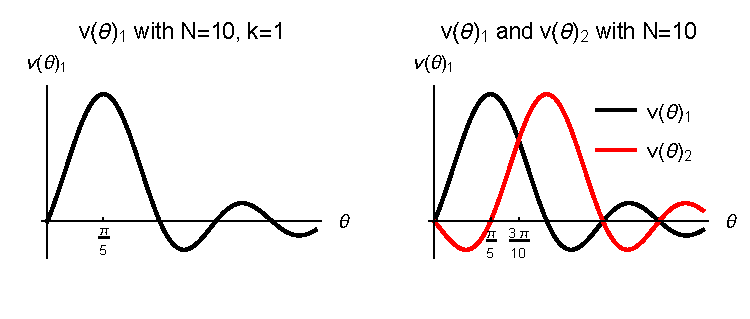
\includegraphics{plot1.pdf}
\end{center}

We can then define projection operators $P_kv_m=\delta_{km}v_m$ and a clock time operator $T_c = \tau\sum{kP_k}$ where $\tau$ is the resolution of the clock. The eigenvectors of $T_c$ are $v_k$ with eigenvalues $t_k = k\tau, k=0,\dots,N-1$. Hence measuring $T_c$ yields discrete approximations to the true time, just as analog and digital clocks do. 

The clock's Hamiltonian is $H_c = \omega J$ where $\omega = \frac{2\pi}{N\tau}$ and $J=-i\hbar \frac{\partial}{\partial\theta}$

The wavefunctions $u_m$ are eigenfunctions of the Hamiltonian:
\[
H_cu_m = m\hbar\omega u_m
\] 

whence expanding the time evolution operator as a Taylor series gives:

\begin{align}
	e^{-\frac{iH_ct}{\hbar}}u_m &= e^{-im\omega t}u_m = (2\pi)^{-\frac{1}{2}}e^{im(\theta-\omega t)} \\
\text{and hence} \\
	\implies e^{-\frac{iH_c\tau}{\hbar}}v_k &= N^{-\frac{1}{2}}\sum_{m}e^{-\frac{2\pi ikm}{N}}e^{-\frac{2\pi im}{N}}u_m \\
						       &= N^{-\frac{1}{2}}\sum_{m}e^{-2\pi i \frac{m}{N}(k+1)}u_m \\
						       &= v_{k+1}
\end{align}

\section{Larmor Precession}

We consider the case of scattering in one dimension with particles of mass $m$, spin $\frac{1}{2}$ and kinetic energy $
E = \frac{\hbar^2k^2}{2m}$. The particles move along the y-axis with spins polarised with the x-axis and interact with a rectangular barrier,

\begin{equation}
	V = 
	\begin{cases}
	V_0 & -\frac{d}{2}<y<\frac{d}{2}\\
		0 & \text{otherwise}
	\end{cases}
\end{equation}

A small magnetic field $\vec{B_{0}}$ points along the z-axis and is confined to the barrier. As particles enter the barrier, the magnetic field induces a Larmor precession with frequency $\omega_{L}=\frac{g \mu B_{0}}{\hbar}$, where $g$ is the gyromagnetic ratio, $\mu$ is the absolute value of the magnetic moment. The polarisations of the transmitted and reflected particles are compared with the polarisation of the incident particles.

Particles initially polarised in the x direction obtain a y and z components when tunnelling through the barrier. We know from the Stern-Gerlach experiment that particles polarised int eh x direction can be represented as combinations of particles with z polarisations, $\ket{x; \pm} = \frac{1}{\sqrt{2}}\ket{z;+} \pm \frac{1}{\sqrt{2}}\ket{z;-}$. Outside the barrier, particles have kinetic energy $E$, independent of their spin. Inside the barrier, the kinetic energy differs by the Zeeman contribution $\pm \frac{\hbar \omega_{L}}{2}$. The wavefunction inside the barrier will contain an exponentially decaying term $Exp(\kappa_{\pm})$, where $\kappa_{\pm} = (k^{2}_{0}-k^{2} \pm \frac{m \omega_L}{\hbar})^{\frac{1}{2}}$, where $\kappa = (k_{0}^2-k^2)^{\frac{1}{2}}$ and the sign indicates spin parallel or antiparallel to the field.  

We can approximate this in the small $\omega_L$ limit as
	\begin{align*}
		\kappa_{\pm} &= \left(k^{2}_{0}-k^{2} \mp \frac{m \omega_{L}}{\hbar}\right)^{\frac{1}{2}}\\	
			     &= \kappa \left(1 \mp \frac{m \omega_{L}}{\hbar \kappa^{2}}\right)^{\frac{1}{2}}\\
			     &\approx \kappa \left(1 \mp \frac{m \omega_{L}}{2\hbar \kappa^{2}}\right)\\
			      &= \kappa \mp \frac{m \omega_{L}}{2\hbar \kappa}
	\end{align*}

Here we examine tunnelling through a barrier in a magnetic field. In this case our Hamiltonian is
\begin{equation}
	H = 
	\begin{cases}
	\left(\frac{p^2}{2m} + V_0\right)\mathbb{1}-\left(\frac{\hbar \omega_L}{2}\right) \sigma_z & |y| \leq \frac{d}{2}\\
	\left(\frac{p^2}{2m}\right)\mathbb{1} & |y| \geq \frac{d}{2}
	\end{cases}
	\end{equation}
where $\mathbb{1}$ is the $2 \times 2$ identity matrix and $\sigma_{x}, \sigma_{y}, \sigma_{z}$ are the Pauli spin matrices.

H acts on spinors
\begin{align}
	\psi &= \begin{pmatrix}
		\psi_{+}(y) \\
		\psi_{-}(y)
		\end{pmatrix}
\end{align}

As usual $|\psi_{\pm}(y)|^{2}dy$ is the probability of finding a particle \textit{upon measurement} with spin $\pm \frac{\hbar}{2}$ in the interval $y, y+dy$. We emphasise the 'upon measurement' here as this is an important point of distinction between the orthodox and pilot-wave interpretations addressed in this essay. The incident beam is polarised in the x direction,
\begin{align}
	\psi &= \frac{1}{\sqrt{2}}
	\begin{pmatrix}
	1\\
	1
	\end{pmatrix}
	e^{i k y}
\end{align}
i.e. $\psi$ is an eigenvector of $S_{x}$

H is diagonal in the spinor basis so we can solve the scattering problem for particles with spin $\frac{\hbar}{2}$ and $-\frac{\hbar}{2}$ separately. 
Our wavefunction is of the form
\begin{equation}
	\psi = 
	\begin{cases}
		A_{\pm}e^{i k y} + B_{\pm}e^{-i k y} & y \leq -\frac{d}{2} \\
		C_{\pm}e^{\kappa_{\pm}y} + D_{\pm}e^{-\kappa_{\pm}y} & -\frac{d}{2} \leq y \leq \frac{d}{2} \\
		F_{\pm}e^{i k y} & y \geq \frac{d}{2}
	\end{cases}
\end{equation}

We will soon set $A_{\pm} = 1$, corresponding to 1 particle per ??, but maintain it for now to aid a future calculation. Note there is no $e^{-i k y}$ term on the right of the barrier, as no particles are reflected. 

The effect of the magnetic field $B_0$ is simply to adjust the height of the barrier, $V_0^{'} = V_0 \pm \frac{\hbar \omega_L}{2}$. Hence we can solve the scattering problem initially assuming no magnetic field, and then adjusting our solution by replacing $\kappa$ in the field-free problem with $\kappa_{\pm}$. Our job now is to calculate the wavefunction coefficients A, B, C, D, F using the continuity of the wavefunction and its first derivative at the boundaries.
This is a lengthy calculation but the results are used so frequently that it is necessary to include a derivation. The results are stated here and derived below:

\begin{align}
	F &= T^{\frac{1}{2}}e^{i\Delta\phi}e^{-ikd} & B &= R^{\frac{1}{2}}e^{-\frac{i\pi}{2}}e^{i\Delta\phi}e^{-ikd} \nonumber \\
	C &= \frac{\kappa+ik}{2\kappa}e^{\frac{ikd}{2}}e^{\frac{-\kappa d}{2}}F & D &= \frac{\kappa-ik}{2\kappa}e^{\frac{ikd}{2}}e^{\frac{\kappa d}{2}}F \label{cont0}
\end{align}
where $T$ is t:he transmission probability and $R = 1-T$ is the reflection probability.

First we introduce a new coordinate system so that the boundaries of our barrier become 0, d. Then, denoting our wavefunctions before, inside and after the barrier as $\psi_{1}, \psi_{2}, \psi_{3}$ respectively, we have:

\begin{align}
	\psi_{1} &= Ae^{iky} + Be^{-iky} & \psi_{1}^{'} &= Aike^{iky} - ikBe^{-iky} \\
	\psi_{2} &= Ce^{-\kappa y} + De^{\kappa y} & \psi_{2}^{'} &= -\kappa Ce^{-\kappa y} + \kappa De^{\kappa y} \\
	\psi_{3} &= Fe^{iky} & \psi_{3}^{'} &= ikFe^{iky}
\end{align}

Imposing continuity of the wavefunction and its first derivative at the barrier boundaries:
\begin{align}
	\psi_{1}(0) = \psi_{2}(0) &\implies A+B = C+D \label{cont1}\\
	\psi_{1}^{'}(0) = \psi_{2}^{'}(0) &\implies ikA - ikB = -\kappa C + \kappa D \label{cont2}\\
	\psi_{2}(d) = \psi_{3}(d) &\implies Ce^{-\kappa d} + De^{\kappa d} = Fe^{ikd} \label{cont3}\\
	\psi_{2}^{'}(d) = \psi_{3}^{'}(d) &\implies -\kappa Ce^{-\kappa d} + \kappa De^{\kappa d} = ikF e^{ikd} \label{cont4}
\end{align}

\begin{align}
	ik(\ref{cont1})+(\ref{cont2}) &\implies 2ikA = C(ik-\kappa)+D(ik+\kappa) \label{cont5}\\
	ik(\ref{cont1})-(\ref{cont2}) &\implies 2ikB = C(ik+\kappa)+D(ik-\kappa) \label{cont6}\\
	\kappa(\ref{cont3})-(\ref{cont4}) &\implies 2\kappa Ce^{\kappa d} = Fe^{ikd}(\kappa-ik) \label{cont7}\\
	\kappa(\ref{cont3})+(\ref{cont4}) &\implies 2\kappa De^{\kappa d} = Fe^{ikd}(\kappa+ik) \label{cont8}
\end{align}

Inserting equations (\ref{cont7}) and (\ref{cont8}) into equation (\ref{cont5}) we arrive at:

\begin{align}
	2ikA &= -\frac{(ik-\kappa)^2}{2\kappa}Fe^{(ik+\kappa)d}+\frac{(ik+\kappa)^2}{2p}Fe^{(ik-\kappa)d} \label{cont9} \\
	\implies 4\kappa ikAe^{-ikd} &= F[(k^2-\kappa^2)(e^{\kappa d}-e^{-\kappa d})+2ik\kappa(e^{\kappa d}+e^{-\kappa d})] \label{cont10}\\
				     &= F[2(k^2-\kappa^2)\sinh{\kappa d}+4ik\kappa \cosh{\kappa d}] \label{cont11}
\end{align}

We hence arrive at our first result, the transmission probability $T = \frac{|F|^2}{|A|^2}$:
\[
	T = [1+\frac{(k^2+\kappa^2)^2\sinh^2{\kappa d}}{4k^2\kappa^2}]^{-1}
.\] 

and, by writing $F$ in polar form $F = |F|e^{i\theta}$, the phase change across the barrier:
i
\begin{align}
	F &\propto 4k^2\kappa^2 \cosh{\kappa d}e^{-ikd}+i2k\kappa(k^2-\kappa^2)\sinh{\kappa d}e^{-ikd} \\
	  &\implies \Delta \phi := arg(F) = \arctan\left(\frac{\operatorname{Im}(F)}{\operatorname{Re}(F)}\right) = \arctan\left(\frac{(k^2-\kappa^2)}{2k\kappa}\tanh{\kappa d}\right) \\
	  &\implies Fe^{ikx}\rvert_{x=d}-e^{ikx}\rvert_{x=0} = |F|e^{i\Delta \phi}e^{ik(d-d)}-1 \\
	  \text{and so the phase change} = \Delta \phi
\end{align}

It is clear now why we left the coefficient A explicit, but from now on it will be set to A = 1.

Rearranging (\ref{cont11}) for $F$, we can compare with the final result in (\ref{cont0}) and factorise out $T^\frac{1}{2}$:

\[
	F = T^{\frac{1}{2}}e^{-ikd} \times \frac{(k^2-\kappa^2)i\sinh{\kappa d}+2k\kappa \cosh(\kappa d)}{\sqrt{(k^2+\kappa^2)^2\sinh^{2}{\kappa d}+4k^2\kappa^2}}
\] 
This yields the identification

\begin{align}
	e^{i\Delta\phi} &= \frac{(k^2-\kappa^2)i\sinh{\kappa d}+2k\kappa \cosh{\kappa d}}{\sqrt{(k^2+\kappa^2)\sinh^{2}(\kappa d)+4k^2\kappa^2}} \\
			&= \frac{(k^2-\kappa^2)i\tanh{\kappa d}+2k\kappa}{\sqrt{(k^2-\kappa^2)^2\tanh^2{\kappa d}+4k^2\kappa^2}}
\end{align}

Expanding the left hand side into real and imaginary parts and comparing coefficients we deduce:

\[
	\tan{\Delta\phi} = \frac{(k^2-\kappa^2)\tanh(\kappa d)}{2k\kappa}
\] 

The result for B follows along similar lines and results for C and D follow immediately from equations (\ref{cont7}) and (\ref{cont8}). We note that our final results are independent of the coordinate system used (up to scaling by a multiplicative constant) so the result also holds in our other coordinate system.

\begin{thebibliography}{100}
\bibitem{Goldstein}
Goldstein

\end{thebibliography}
\end{document}
